\let\negmedspace\undefined
\let\negthickspace\undefined
%\RequirePackage{amsmath}
\documentclass[journal,12pt,twocolumn]{IEEEtran}
 \usepackage[utf8]{inputenc}
 \usepackage{graphicx}
 \usepackage{amsmath}
 \usepackage{mathrsfs}
\usepackage{txfonts}
\usepackage{stfloats}
\usepackage{bm}
\usepackage{cite}
\usepackage{cases}
\usepackage{subfig}
 \usepackage{amsfonts}
 \usepackage{amssymb}
 \usepackage{enumitem}
\usepackage{mathtools}
\usepackage{tikz}
\usepackage{circuitikz}
\usepackage{verbatim}
\usepackage[breaklinks=false,hidelinks]{hyperref}
\usepackage{listings}
\usepackage{calc}
\usepackage{float}
\usepackage{longtable}
\usepackage{multirow}
\usepackage{multicol}
\usepackage{color}
\usepackage{array}
\usepackage{hhline}
\usepackage{ifthen}
\usepackage{chngcntr}
\usepackage{url}
\def\UrlBreaks{\do\/\do-}

\lstset{frame=single,breaklines=true,columns=fullflexible}

\newcommand{\BEQA}{\begin{eqnarray}}
\newcommand{\EEQA}{\end{eqnarray}}
\newcommand{\define}{\stackrel{\triangle}{=}}
\bibliographystyle{IEEEtran}
%\bibliographystyle{ieeetr}
\def\inputGnumericTable{}
\DeclareMathOperator*{\Res}{Res}
\let\vec\mathbf
\numberwithin{equation}{section}
\renewcommand\thesection{\arabic{section}}
\renewcommand\thesubsection{\thesection.\arabic{subsection}}
\renewcommand\thesubsubsection{\thesubsection.\arabic{subsubsection}}

\renewcommand\thesectiondis{\arabic{section}}
\renewcommand\thesubsectiondis{\thesectiondis.\arabic{subsection}}
\renewcommand\thesubsubsectiondis{\thesubsectiondis.\arabic{subsubsection}}

\providecommand{\pr}[1]{\ensuremath{\Pr\left(#1\right)}}
\providecommand{\sbrak}[1]{\ensuremath{{}\left[#1\right]}}
\providecommand{\lsbrak}[1]{\ensuremath{{}\left[#1\right.}}
\providecommand{\rsbrak}[1]{\ensuremath{{}\left.#1\right]}}
\providecommand{\brak}[1]{\ensuremath{\left(#1\right)}}
\providecommand{\lbrak}[1]{\ensuremath{\left(#1\right.}}
\providecommand{\rbrak}[1]{\ensuremath{\left.#1\right)}}
\providecommand{\cbrak}[1]{\ensuremath{\left\{#1\right\}}}
\providecommand{\lcbrak}[1]{\ensuremath{\left\{#1\right.}}
\providecommand{\rcbrak}[1]{\ensuremath{\left.#1\right\}}}
\providecommand{\abs}[1]{\left\vert#1\right\vert}
\providecommand{\res}[1]{\Res\displaylimits_{#1}}
\newcommand{\myvec}[1]{\ensuremath{\begin{pmatrix}#1\end{pmatrix}}}
\newcommand{\mydet}[1]{\ensuremath{\begin{vmatrix}#1\end{vmatrix}}}

\newcommand{\question}{\noindent \textbf{Question: }}
\newcommand{\solution}{\noindent \textbf{Solution: }}

\providecommand{\link}[2]{{\color{blue}\href{https://github.com/SterbenVD/AI1110-Assignments/Assignment/#1}{#2}}}

\title{Assignment: Random Numbers}
\author{Vishal Vijay Devadiga (CS21BTECH11061)}
\date{}
\begin{document}
% make the title area
\maketitle

\section{Uniform Random Numbers}
Let $U$ be a uniform random variable between 0 and 1.
\begin{enumerate}[label=\thesection.\arabic*,ref=\thesection.\theenumi]
\item Generate $10^6$ samples of $U$ using a C program and save into a file called uni.dat.
\\
\solution Download the following files and execute the \link{codes/1-1.c}{C program}.
\\
\item
Load the uni.dat file into python and plot the empirical CDF of $U$ using the samples in uni.dat. 
The CDF is defined as:
\begin{align}
F_{U}(x) = \pr{U \le x}
\end{align}
\begin{figure}[H]
\centering
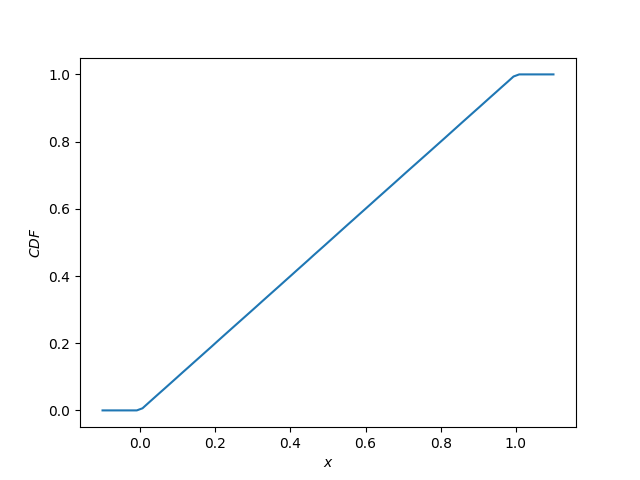
\includegraphics[width=\columnwidth]{../figs/1_cdf.png}
\caption{The CDF of $U$}
\label{fig:1_cdf}
\end{figure}
\solution  The following \link{codes/1-2.py}{python code} plots Fig. \ref{fig:1_cdf}
\\
\item Find a  theoretical expression for $F_{U}(x)$.
\\
\solution
\\
\item
The mean of $U$ is defined as:
\begin{equation}
E\sbrak{U} = \frac{1}{N}\sum_{i=1}^{N}U_i
\end{equation}
and its variance as:
\begin{equation}
\text{var}\sbrak{U} = E\sbrak{U- E\sbrak{U}}^2 
\end{equation}
Write a C program to  find the mean and variance of $U$.
\\ 
\solution Download the following files and execute the \link{codes/1-3.c}{C program}.
\\
\item Verify your result theoretically given that:
\begin{equation}
E\sbrak{U^k} = \int_{-\infty}^{\infty}x^kdF_{U}(x)
\end{equation}
\solution
\end{enumerate}

\section{Central Limit Theorem}
\begin{enumerate}[label=\thesection.\arabic*,ref=\thesection.\theenumi]
\item Generate $10^6$ samples of the random variable:
\begin{equation}
X = \sum_{i=1}^{12}U_i -6
\end{equation}
using a C program, where $U_i, i = 1,2,\dots, 12$ are  a set of independent uniform random variables between 0 and 1
and save in a file called gau.dat.
\\
\solution Download the following files and execute the \link{codes/2-1.c}{C program}.
\\
\item Load gau.dat in python and plot the empirical CDF of $X$ using the samples in gau.dat. What properties does a CDF have?

\begin{figure}[H]
\centering
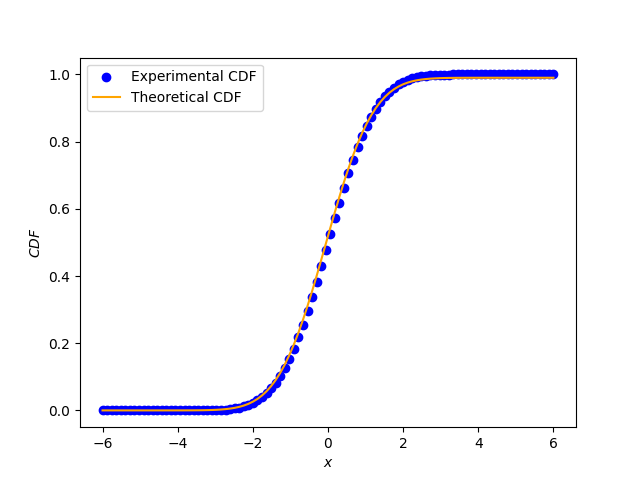
\includegraphics[width=\columnwidth]{../figs/2_cdf}
\caption{The CDF of $X$}
\label{fig:2_cdf}
\end{figure}
\solution The following \link{codes/2-2.py}{python code} plots Fig. \ref{fig:2_cdf}
\\
\item Load gau.dat in python and plot the empirical PDF of $X$ using the samples in gau.dat. 
The PDF of $X$ is defined as:
\begin{align}
p_{X}(x) = \frac{d}{dx}F_{X}(x)
\end{align}
What properties does the PDF have?
\begin{figure}[H]
    \centering
    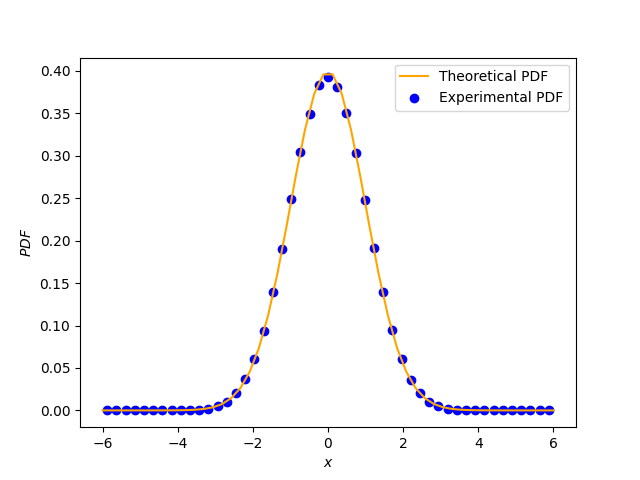
\includegraphics[width=\columnwidth]{../figs/2_pdf}
    \caption{The PDF of $X$}
    \label{fig:2_pdf}
\end{figure}
\solution The following \link{codes/2-3.py}{python code} plots Fig. \ref{fig:2_pdf}
\\
\item Find the mean and variance of $X$ by writing a C program.
\\
\solution Download the following files and execute the \link{codes/2-3.c}{C program}.
\\
\item Given that:
\begin{align}
p_{X}(x) = \frac{1}{\sqrt{2\pi}}\exp\brak{-\frac{x^2}{2}}, -\infty < x < \infty,
\end{align}
repeat the above exercise theoretically
\\
\solution Download the following files and execute the \link{codes/2-4.c}{C program}.
\end{enumerate}

\section{From Uniform to Other}
\begin{enumerate}[label=\thesection.\arabic*,ref=\thesection.\theenumi]
\item
Generate samples of:
\begin{equation}
V = -2\ln\brak{1-U}
\end{equation}
and plot its CDF.
\\
\solution Download the following files and execute the \link{codes/3-1.c}{C program} to generate the samples. \\
The following \link{codes/3-1.py}{python code} plots Fig. %\ref{fig:3_cdf}
%\begin{figure}[H]
%\centering
%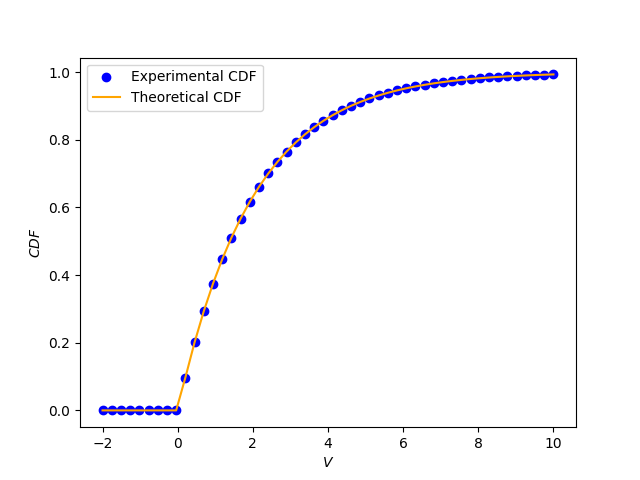
\includegraphics[width=\columnwidth]{../../figs/3_cdf}
%\caption{The CDF of $X$}
%\label{fig:3_cdf}
%\end{figure}
\\
\item Find a theoretical expression for $F_V(x)$.
\\
\solution
\end{enumerate}
\end{document}